% !TEX encoding = UTF-8
% !TEX TS-program = pdflatex
% !TEX root = ../tesi.tex

%**************************************************************
\chapter{Introduzione}
\label{cap:introduzione}
%**************************************************************

In questo capitolo viene descritta l'azienda, le metodologie utilizzate e come viene organizzato il lavoro. \\

%\noindent Esempio di utilizzo di un termine nel glossario \\
%\gls{api}. \\

%\noindent Esempio di citazione in linea \\
%\cite{site:agile-manifesto}. \\

%\noindent Esempio di citazione nel pie' di pagina \\
%citazione\footcite{womak:lean-thinking} \\

%**************************************************************
\section{L'azienda}

Sync Lab nasce nel 2002 come Software house e si è trasformata rapidamente in System Integrator attraverso uno studiato processo di maturazione delle competenze tecnologiche, metodologiche ed applicative nel dominio del software.
\\
\begin{figure}[htbp]	
		\centering
		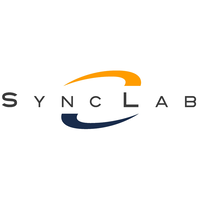
\includegraphics[width=7cm]{immagini/logo.png}
		\caption{Logo aziendale Sync Lab}
		\label{fig:Logo aziendale Sync Lab}
\end{figure}
\\
\\
In seguito all'apertura della sede principale di Napoli, Sync Lab è cresciuta esponenzialmente nel mercato ICT e ha consolidato ottimi rapporti con clienti e partner.
Attualmente l'aziende ha più di 150 clienti diretti e finali e vanta un organico di oltre 200 dipendenti, una solida base finanziaria e un'ottima diffusione nel territorio italiano attraverso le sue cinque sedi: Napoli, Roma, Milano, Padova e Verona.
\\
\begin{figure}[htbp]	
	\centering
	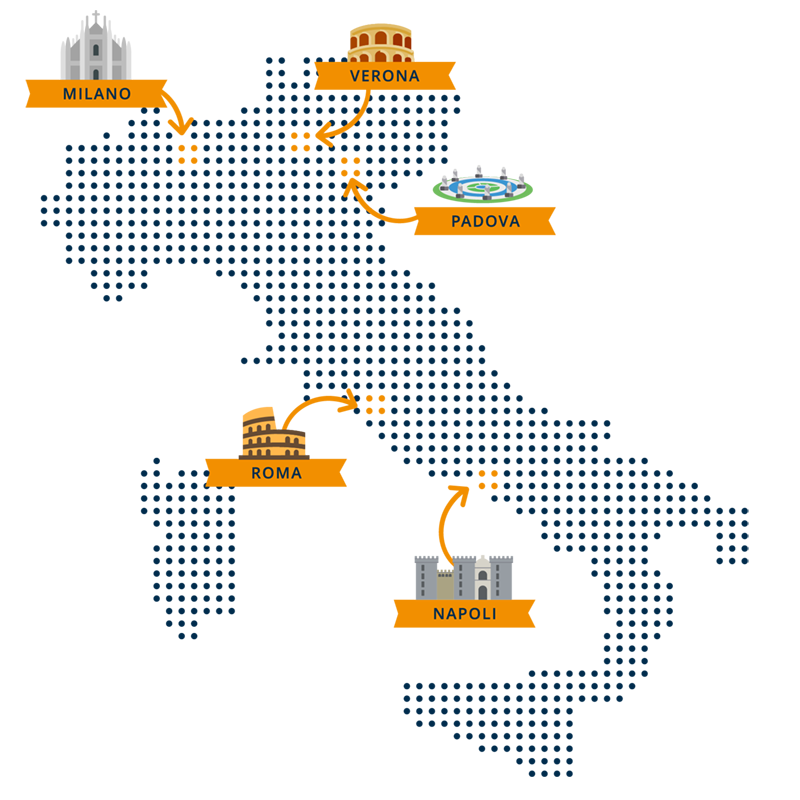
\includegraphics[width=8cm]{immagini/sedi.png}
	\caption{Sedi Sync Lab}
	\label{fig:Sedi Sync Lab}
\end{figure}
\\
Sync Lab, propone sul mercato interessanti e innovativi prodotti software, nati nel proprio laboratorio di ricerca e sviluppo. Attraverso questi prodotti, Sync Lab ha gradualmente conquistato significativamente fette di mercato nei seguenti settori: mobile, videosorveglianza e sicurezza delle infrastrutture informatiche aziendali.

%**************************************************************
\section{Metodologie utilizzate e principali prodotti}
L’azienda adotta un modello di sviluppo agile che pone le proprie basi nel metodo Scrum. Gli stakeholders, infatti, vengono costantemente coinvolti nel processo di
sviluppo del prodotto per raccogliere feedback. Gli obiettivi si possono riassumere in tre punti fondamentali:
\begin{itemize}
	\item Comprendere attentamente il contesto operativo del cliente; 
	\item Fornire al cliente un supporto mirato; 
	\item Accelerare e favorire la formazione di soluzioni. 
\end{itemize}
In base a questi principi Sync Lab raggiunge i propri obiettivi grazie a:
\begin{itemize}
	\item Consulenza; 
	\item Fornitura; 
	\item Sviluppo; 
	\item Manutenzione. \\
\end{itemize}

Nell'ambito di prodotti e innovazioni, l'azienda ne può vantare un buon numero.
Tra questi troviamo: 
\begin{itemize}
	\item \textbf{SynClinic} che è un  software integrato per la gestione delle strutture sanitarie, che permette di gestire, organizzare e monitorare tutte le fasi del percorso di cura del paziente; \\
	\begin{figure}[htbp]	
		\centering
		
\includegraphics[width=7cm]{immagini/synClinic.jpg}
		\caption{SynClinic}
		\label{fig:SynClinic}
	\end{figure}
	\\
	\item \textbf{DPS 4.0} che permette di gestire la General Data Protection Regulation(GDPR) Privacy in pochi semplici passi con una soluzione guidata per aggiornare e modificare i documenti di privacy in modo conforme agli standard di riferimento; \\
	\item \textbf{StreamLog} che permette di gestire la compliance al provvedimento del Garante per la protezione dei dati personali relativo agli Amministratori di Sistema (AdS). In particolare, permette di soddisfare requisiti fissati dal Garante; \\
	\item \textbf{StreamCrusher} che è una tecnologia che aiuta ad essere bene informati su quando bisogna prendere decisioni di business, ad identificare velocemente criticità ed a riorganizzare i processi in base a nuove esigenze; \\
	\item \textbf{Wave} che si propone come integrazione tra i mondi della Videosorveglianza e quello dei Sistemi Informativi Territoriali (GIS) abilitando il controllo totale dell'area da sorvegliare; \\
	\item \textbf{Seastream} che mette a disposizione un sistema di monitoraggio avanzato delle flotte armatoriali operative in tutto il mondo e una piattaforma integrata di servizi per gli operatori in ambito portuale. \\
\end{itemize}



%**************************************************************

